\documentclass[preprint,natbib209]{aastex}
\usepackage{url}
\usepackage{amsmath}
\usepackage{amssymb}
\usepackage{afterpage}
\slugcomment{To be submitted to \apj\ or \mnras}
\shorttitle{Physically Properties of Serendipitous sub-mm Galaxies}
\shortauthors{Hagen et al.}
\newcommand{\eg}{e.g.}
\citestyle{apj}
\begin{document}

\title{Heterogeneous Physical Properties of Serendipitously Discovered Galaxies: 
Low-mass sub-millimeter galaxies and others at $0.6 < z < 3$}

\author{Alex Hagen\altaffilmark{1,2,3}}
\affil{Department of Astronomy \& Astrophysics, The Pennsylvania State 
University, 525 Davey Lab, University Park, PA 16802}
\email{hagen@psu.edu}

\author{Seiji Fujimoto, Masami Ouchi}
\affil{Institute for Cosmic Ray Research, The University of Tokyo, Kashiwa 277 8582, Japan}
\email{sfseiji@icrr.u-tokyo.ac.jp, ouchims@icrr.u-tokyo.ac.jp}

\author{et al.}

\altaffiltext{1}{Institute for Gravitation and the Cosmos, The Pennsylvania State University, University Park, PA 16802}
\altaffiltext{2}{NSF East Asia and Pacific Summer Institute Fellow 2015}
\altaffiltext{3}{Institute for Cosmic Ray Research, The University of Tokyo, Kashiwa 277 8582, Japan}

\begin{abstract} 

\end{abstract}
\keywords{galaxies: evolution -- galaxies: high-redshift -- cosmology: observations}

%\begin{figure}[htpb]
%	\centering
%	\includegraphics[scale=0.4]{fitting.pdf}
%	trim = left bottom right top
%	\caption{The given data and both fits. The Gaussian is a clearly a better fit than the Lorentzian}
%	\label{fit}
%\end{figure}
%\citep[e.g.,][]{verhamme12, yajima12, behrens14}

\section{Introduction}
\label{sec:intro}

Traditional sub-millimeter galaxies sample galaxies sample very dusty, highly star forming galaxies at high redshift \citep[e.g.][and references therein]{blain02, lagache05, casey14, lutz14}. These galaxies, as referred to as dusty star-forming galaxies (DSFG) to reference their physical properties instead of a possible detection technique, are some of the most intensely star forming galaxies in the known universe. Their discovery across redshifts is due to the Rayleigh-Jeans tail of the dust blackbody curve almost perfectly cancelling out cosmological dimming from $1 \lesssim z \lesssim 8$ in the wavelength range of $850\text{$\mu$m} \lesssim \lambda \lesssim 2\text{mm}$ \citep[See][Figure 3]{casey14}; this is referred to as the ``negative K correction."

Traditionally, SMGs were found with single-dish telescopes, which limited the resolution and thus made follow-up difficult. The addition Atacama Large Millimeter Array has given sub arcsecond resolution at sub-millimeter wavelengths, allowing for unprecedented studies of SMGs. The ALMA LABOCA ECDFS Submillimeter \citep[ALESS;][]{hodge13} used ALMA to study SMGs selected in the Extended Chandra Deep Field South. \cite{dacunha15} showed that these ALESS SMGs have a wide range of physical properties, including some that have significantly less dust attenuation than expected; furthermore, half of these galaxies are above the stellar mass -- star formation rate relation, while the other half match the relation. \cite{dunlop16} examined the first deep ALMA image of the Hubble Ultra Deep Field and found a large range of stellar masses, redshifts, and physical properties. This shows that SMGs are not just star-bursting galaxies, but cover a wide range of properties. 

This paper focuses on galaxies first discussed in \cite{fujimoto16} serendipitously selected via deep 1.2mm archival ALMA observations. 
Studying these serendipitous sub-mm selected galaxies is important to understand the whole population of galaxies with sub-mm emission.
While classical SMGs are rare and in highly biased regions, F16 found that the bias of these galaxies was significantly lower than that of traditional SMG and pBzK galaxies, and similar to those of sBzKs, LBGs, and LAEs. This study provides the opportunity to understand the physical properties of these galaxies. By understanding this we can further understand the sub-mm emission for less biased, more commonly found sub-mm galaxies, and improve our understanding of the physical properties of these galaxies.

We adopt the standard concordance cosmology of $h = 0.7$, $\Omega_m = 0.3$, $\Omega_\Lambda = 0.7$, 
and $\Omega_k = 0$ \citep{planck13}.

\section{Sample Selection} 
\label{sec:sample}

Our sample comes from \citet{fujimoto16}, hereafter F16, who studied serendipitously discovered sub-mm galaxies in 
120 deep ALMA pointings pulled from the ALMA archive. This work achieved depths of 0.05 mJy at 1.2mm in the field and 0.02 mJy 
with the assistance of gravitational lensing in A1689; it discovered a total of 133 galaxies. Many of the ALMA observations in F15 were not
in deep fields with ancillary photometry sufficient to identify counterparts. Thus, F16 focused on identifying counterparts in Subaru XMM-Newton Deep 
Survey \citep[SXDS;][]{furusawa08} and Abel 1689 (A1689), both of which are covered by multi-wavelength surveys. 
Out of 65 serendipitous ALMA sources, F16 identified 17 counterparts -- 2 in A1689 and 15 in SXDS. Of these, 12 have enough counterpart photometry to accurately find a photometric redshift so SED fitting can be done.

We also visually inspected the counterparts and determined that S2 is a blend of two faint sources, S7 is also between two sources, and that S9 looks to be a star, as it is relatively bright and a PSF

%% add in cosmos counterparts
%To ensure were were not missing any counterparts, we searched for counterparts for each galaxy in The NASA Extragalactic Data (NED), and
%the \textit{Hubble} Source Catalog (HSC; Whitmore et al., in prep). This led us to discover YY new optical counterparts, 
%mostly in the COMOS field \citep{COSMOS}. %have a table of new counterparts? and maybe a table of photometry?
We identified an optical counterpart for F16 source ID 7 originally found in the HSC and the Sloan Digital Sky Survey \citep[SDSS;][]{york2000} 
DR12 \citep{alam15} imaging data \citep{fukugita96, gunn98, hogg01, smith02, pier03, ivezic04, gunn06, tucker06, padmanabhan08, doi10}.

The photometry for the counterparts identified in F16 comes from a variety of multi-wavelength surveys in SXDS and A1689.
In SXDS we use the following bands \textit{u*} (Foucaud et al., in prep.), \textit{B, V, R, i', z'} \citep{furusawa08},
\textit{J, H, K} \citep[UKIDSS;\footnotemark][]{lawrence07} 3.6 - 24 $\mu$m \citep[SWIRE, SpUDS, SEDS;][]{lonsdale03, ashby13}
250 - 500 $\mu$m \citep[HerMES;][]{oliver12, smith12, wang14} and 1.4 GHz \citep{simpson06}.
In A1689 we use \textit{g$_{475}$, r$_{625}$, i$_{775}$, z$_{850}$, J$_{110}$} \& \textit{H}$_{160}$ from the HSC,
 3.6 - 24 $\mu$m from \textit{Spitzer} Enhanced Imaging Products (SEIP), and 250 - 500 $\mu$m (HerMES).

\footnotetext{The UKIDSS project is defined in \citet{lawrence07}. UKIDSS uses the UKIRT 
Wide Field Camera \citet[WFCAM][]{casali07}. The photometric system is described in 
\citet{hewett06}, and the calibration is described in \citet{hodgkin09}. 
The pipeline processing and science archive are described in \citet{hambly08}.}

\section{Analysis}
\label{sec:analysis}

%talk about how important it is to have consistency in whole fit -- energy extinguished from dust heats dust, so there's energy balance
We use spectral energy distribution fitting (SED fitting) to infer physical properties of our sample of galaxies \citep[for a recent review of SED fitting see][]{conroy13}. It is of great importance to have energy balance in our SED fitting; the energy of the starlight attenuated by dust is reprocessed and emitted in the infrared. It is normally quite difficult to measure the dust emission, particularly in low-mass galaxies, and our sample of galaxies are selected in such a way that its possible to do this. Balancing the dust emission with the dust absorption allows for the degeneracy between age and dust attenuation, common in SED fitting that only doesn't include mid- and far-IR, to be broken. This allows for a better estimation of the star formation history as well.

\subsection{Software Choice}
We used two different software packages to model the SEDs of our galaxies, \texttt{Multi-wavelength Analysis of Galaxy Physical Properties} (MAGPHYS) \citep{dacunha08, dacunha15} and \texttt{Flexible Stellar Population Synthesis} (FSPS) \citep{conroy09, conroy10}. Both of these packages generate SEDs with inputs of physical parameters and stellar isochrones; the best-fit physical parameters and their uncertainties are found by maximizing the likelihood, using a Bayesian approach by taking priors into account when an informed prior can be found. MAGPHYS builds up the marginalized likelihood for each parameter by comparing the data to all combinations of models in a grid search. For FSPS we used a the \texttt{emcee} Markov Chain Monte Carlo package \citep{emcee} coupled with the \texttt{python-fsps} interface to \texttt{FSPS} \citep{python-fsps}. For more detail on the python wrapper software for FSPS, see Hagen et al. (2016b, in prep). 

In our use of \texttt{FSPS}, we found that the outputs could not be used for further analysis, as we hit an edge in the parameter distribution for the strength of the radiation field. The dust emission models used in \texttt{FSPS}, from \cite{draine07}, allow the strength of the radiation field go to twenty-five times the Milky Way level. The output distributions for all galaxies consistently hit the edge of this range, meaning that our results our biased as there are well-fitting models that lie outside the range of the \texttt{FSPS} software. While we do not use the physical parameter outputs, there is still a lesson to be learned here -- the radiation field intensities in these galaxies are very high compared to the Milky Way. This is consistent with their compact nature and star formation rates. We also hope that this finding provides motivation to increase the parameter range in the dust emission models in \texttt{FSPS}.

\subsection{MAGPHYS}

We use \texttt{Magphys} for SED fitting for the rest of this paper. In particular, we use the version of \texttt{Magphys} for high-z galaxies, as described by \cite{dacunha15}.  We will briefly summarize the \texttt{Magphys} approach here; for more details, see Sections 3 \& 4 of \cite{dacunha15} 
\texttt{Magphys} uses a library of 50,000 stellar models adapted for modeling high-z galaxies. The \cite{dacunha15} high-z extension to \texttt{Magphys} has added high dust opacities, higher star formation rates, and younger ages. Note that the code also includes low dust opacities, low SFRs, and old ages so it does not bias itself. 

\texttt{Magphys} uses the \cite{bruzual07} updated versions of the \cite{bruzual03} stellar population synthesis models. Dust attenuation is computed using the two component model of \cite{charlot00}; this model applies an additional ``birth-cloud" opacity for stars younger than $10^7$ years. The shape of the dust law is a power law as detailed in \cite{charlot00}. 

The star formation history is split into two parts -- a continuos SFR and stochastic bursts. The continuous SFH is a continuous delayed exponential of the form $\psi \propto \gamma^2 t \exp \left( -\gamma t \right)$ where $t$ is the time since the onset of star formation and $\gamma = \frac{1}{\tau_{SF}}$.  This form of the star formation history is quite flexible and physically motivated, as it rises in early times, flattens out, and then exponentially declines. Thus it can match everything from the increasing SFR for very young galaxies to the decreasing SFR of older galaxies. The parameter range of $\gamma$ is very broad, so that the peak of SFR can happen anywhere from 0.7-13.3 Gyr after the onset of star formation. Accounting for stochastic bursts is done by imposing random bursts on top of the continuous SFH. The bursts can last from 30-300 Myr and can vary in strength from 0.1-100 times the continuous SFH. \cite{dacunha15} states ``We set the probability of a burst of star formation occurring at any random time in the previous 2 Gyrs to 75\%." Including the stochastic bursts allows for \texttt{Magphys} to account for a much broader range of possible star formation histories than a simple continuous function with adding additional parameters.

The dust emission is modeling using four components: empirical templates for polycyclic aromatic hydrocarbons (PAHs), mid-IR continuum for hot dust, warm dust (30 - 80 K in stellar birth clouds) in thermal equilibrium, and cool dust (20 - 40 K in the diffuse ISM) in thermal equilibrium. The strengths of these four components are floating parameters in the model. The SED of the dust in thermal equilibrium follows a modified blackbody curve of the form $\nu^{\beta} B_\nu (T)$ where $\beta = 1.5$ for warm dust and $\beta = 2.0$ for cool dust. \cite{dacunha15} also notes that, while the empirical PAH templates may not match SMG PAH emission precisely, the typical PAH contribution to the total dust emission is $< 10\%$ and so uncertainties in the PAH templates won't have a large effect on the results.

The actual SED fitting in \texttt{Magphys} is done by generating model spectra at the redshift of the galaxy in question. These are convolved with filters and compared to the observed data. The log likelihood of a particular model is $-\chi^2 / 2$ (under assumptions of Gaussian uncertainties), and the likelihoods of each parameter are built up through comparison of all the generated models. We note that the Bayesian nature of this code returns the distributions, not just best-fit values, for each model parameter. This is incredibly important, as degeneracies in SED fitting, particularly with large numbers of parameters, are quite common. Being able to explore the distribution enables us to understand how constrained each particular parameter is.

\subsection{Photometric Redshifts}

Only one galaxy, F16's A1, had a spectroscopic redshift. For all others, photometric redshifts were found using \cite{eazy}.

\section{Results}
\label{sec:results}

The SED fitting results are shown in Table \ref{table:sed}. Figure \ref{fig:allsed} compares the best-fit SED for each galaxy in our sample. This cleanly demonstrates the main point of our work -- serendipitously selected sub-mm galaxies cover a wide range of physical properties. While some follow a scaled down SED of a traditional SMG, others are optically bright and look like continuum selected star forming galaxies. These serendipitous sources allow us to include far-IR and radio observations into sources that have never been studied in this way. 

%%%%results table here with same columns as da cunha 15?
\begin{deluxetable}{ccccccc}
\tabletypesize{\footnotesize}
\tablewidth{0pt}
\tablecaption{SED Fitting Results \label{table:sed}}
\tablehead{
\colhead{Galaxy ID} & \colhead{Redshift} & \colhead{Log Stellar Mass} & \colhead{Log SFR} & \colhead{$A_V$} & \colhead{$T_{Dust}$} & \colhead{Log Dust Mass} }
\startdata
A1 & 2.60 & $9.25_{-0.09}^{+0.115}$ & $1.20_{-0.04} ^{+0.07}$ & $2.31_{-0.1} ^{+0.05}$& $49_{-5}^{+5}$ &  $7.33_{-0.10} ^{0.10}$   \\
F7 & 0.677 & $9.97_{-0.23} ^{+0.24}$ & $1.12_{-0.26} ^{+0.30}$ &$0.64_{-0.33} ^{+0.48}$ & $47_{-10}^{+11}$&   $7.07_{-0.36} ^{0.26}$     \\
S1 & 1.377 &  $11.18_{-0.01} ^{+0.01}$  & $1.18_{-0.01} ^{+0.01}$ &$0.56_{-0.01} ^{+0.01}$ & $36_{-7}^{+8}$&       $8.28_{-0.22} ^{0.12}$        \\
S3 & 2.328 &  $9.877_{-0.07} ^{+0.01}$ & $1.73_{-0.01} ^{+0.1}$ &$1.79_{-0.01} ^{+0.01}$ &$64_{-3}^{+6}$ &    $7.06_{-0.07} ^{0.12}$       \\
S4 & 1.569 & $10.47_{-0.01} ^{+0.09}$ & $0.43_{-0.01} ^{+0.14}$ &$0.46_{-0.08} ^{+0.08}$ &$33_{-4}^{+7}$ &     $7.52_{-0.31} ^{0.20}$          \\
S5 & 2.939 & $9.41_{-0.01} ^{+0.02}$ & $1.20_{-0.01} ^{+0.1}$ &$0.24_{-0.01} ^{+0.18}$ &$41_{-6}^{+13}$ &     $7.35_{-0.26} ^{0.22}$       \\
S6 & 0.442 &   $10.87_{-0.01} ^{+0.01}$  & $0.41_{-0.01} ^{+0.01}$ &$1.84_{-0.01} ^{+0.01}$ &$40_{-3}^{+1}$ &   $6.57_{-0.11} ^{0.21}$             \\
S10 & 0.82 & $9.03_{-0.06} ^{+0.06}$  & $0.07_{-0.45} ^{+0.01}$ &$1.29_{-0.53} ^{+0.01}$ &$44_{-9}^{+12}$ &    $6.19_{-0.19} ^{0.65}$           \\
S11 & 1.876 &  $11.73_{-0.01} ^{+0.01}$ & $2.30_{-0.01} ^{+0.01}$ &$2.06_{-0.01} ^{+0.01}$ & $64_{-3}^{+1}$&      $7.78_{-0.01} ^{0.13}$      \\
S12 & 1.561 &  $11.55_{-0.01} ^{+0.01}$  & $1.94_{-0.01} ^{+0.01}$ &$0.99_{-0.01} ^{+0.01}$ & $55_{-13}^{+4}$&    $8.08_{-0.74} ^{0.15}$          \\
%S2 & 1.955 & $8.39_{-0.01} ^{+0.32}$  & $-0.12_{-0.01} ^{+0.01}$ &$0.01_{-0.01} ^{+0.01}$ & $50_{-12}^{+14}$&    $6.00_{-0.01} ^{0.01}$         \\
%S7 & 1.589 &  $8.00_{-0.01} ^{+0.01}$  & $-0.44_{-0.1} ^{+0.15}$ &$0.24_{-0.1} ^{+0.15}$ & $49_{-12}^{+14}$&     $6.00_{-0.01} ^{0.01}$            \\
%S9 & 0.665 &  $10.74_{-0.1} ^{+0.01}$ & $-1.25_{-0.01} ^{+0.04}$ &$0.11_{-0.03} ^{+0.01}$ & $34_{-6}^{+6}$&     $6.00_{-0.01} ^{0.47}$           \\
\enddata
\tablecomments{All uncertainties shown are the 16th and 84th percentiles of the distribution. The IDs are from F16. The redshifts are all photometric redshifts, except A1, which is spectroscopic. The units of stellar mass and dust mass are log solar masses. Star formation rate is in units of log solar masses per year. $A_V$ is measured in magnitudes, and $T_{Dust}$ is measured in Kelvin. Note that $T_{Dust}$ is the luminosity weighted dust temperature (see equation 8 of \cite{dacunha15}), and not the cold dust temperature. The best fit cold dust temperature for all our galaxies is $\sim 25$K.}
\end{deluxetable}


\begin{figure}[t]
\centering
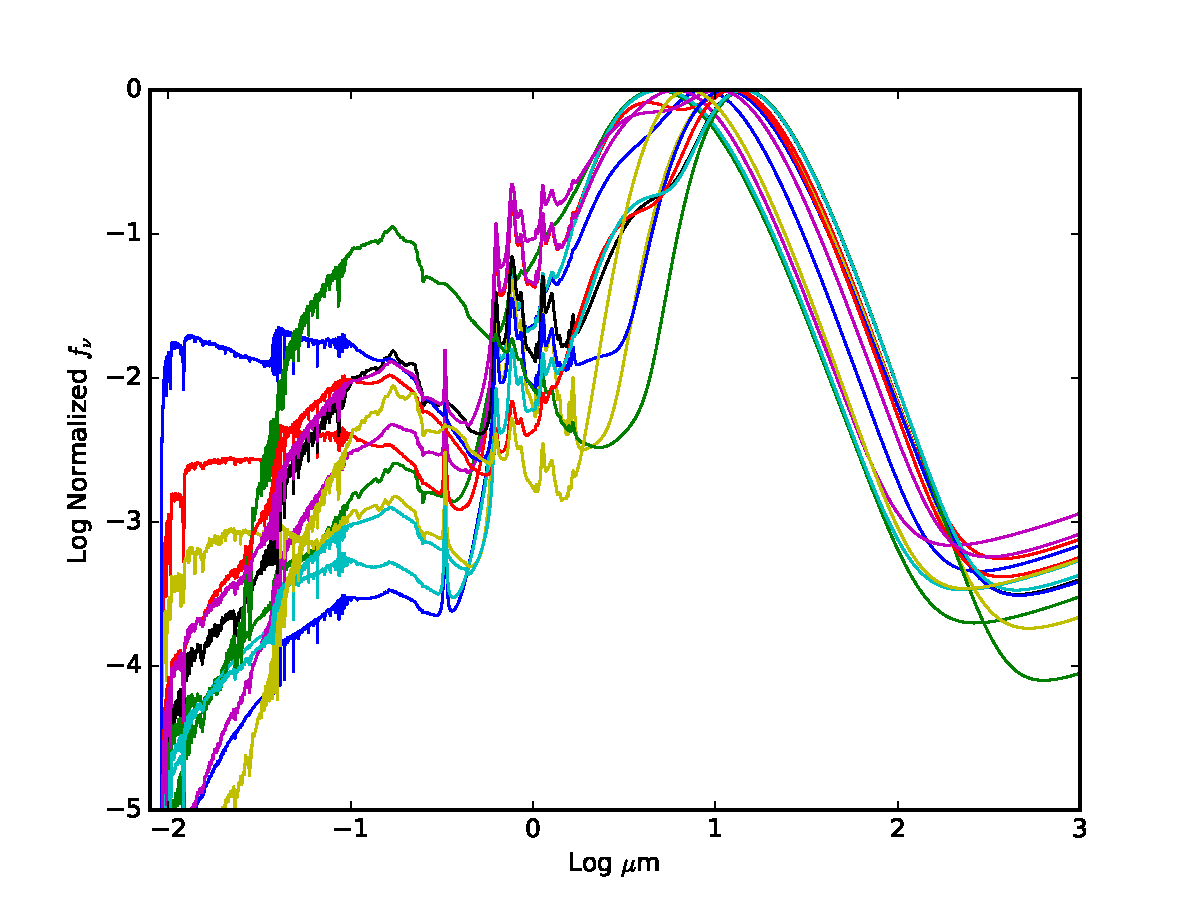
\includegraphics[scale=0.8]{all_sed.pdf}
\caption{Normalized log $f_\nu$ for the best fit SED for each object. These galaxies how a large variety of physical properties inferred from their SEDs. Some galaxies are bright in the UV/optical and some are very extinguished. Some galaxies have bright PAH emission features while some are very faint. The large range of dust temperatures can be seen in the shifts of the peak of the cold dust emission spectrum. These serendipitously selected sub-mm galaxies have a large variety of SEDs, as opposed to traditional SMGs. This demonstrates that this galaxy selection technique is a way to probe dust conditions across a wide variety of galaxies.}
\label{fig:allsed}
\end{figure}

\subsection{Comparison Samples}
To put these galaxies in context, we have selected four different comparison samples to appear in plots of physical properties as allows. The first is the ALESS sample of \cite{dacunha15}. This sample is made of traditionally selected sub-mm galaxies, although the results from this paper also show a broader range of physical properties than was expected. This sample allows us to compare our galaxies to other sub-mm selected galaxies.

We also use a second sample of sub-mm selected galaxies from \cite{dunlop16}, also referred to as D16 in this paper. While the ALESS sample was originally detected by at $870 \mu$m and then follow-up using ALMA, the D16 sample was ALMA-selected. The ALMA observations used in D16 were significantly deeper than those from the ALESS survey and thus these two works together compliment each other in providing physical properties of different selected SMGs.

The third sample is the $1.9 < z < 2.35$ optical emission line selected sample from \cite{zeimann14}. We refer to these galaxies as optical emission line galaxies (oELGs). This sample was selected for strong emission lines in 3DHST grism observations. We chose this sample as it also selected star forming galaxies, but with low reddenings. It also extends to much fainter masses than the released 3DHST catalogs, which is useful as we also have very low mass galaxies. 

Our fourth and final sample is the continuum selected sample from \cite{kurczynski16}, also referred to as K16. These galaxies were selected via the UVUDF and CANDELS imaging and go to very low mass limits. We particularly adopt the sample from $2 < z < 2.5$ as this matches well with our sample.

These four samples bracket our sample in selection methods and physical properties. With this we can put our sub-mm selected galaxies in context, instead of engaging in galaxy ``stamp collecting."

\subsection{Physical Property Results}

Figure \ref{fig:mass_comp} shows the stellar mass comparison between our sample and the four comparison samples. Our sample covers 4+ dex in stellar mass and is bracketed by the comparison samples. The closest sample is that of D16. Some of these galaxies fit in the ALESS stellar mass range and others have similar masses to the oELGs. This large stellar mass range also implies that this selection is samples across a wide range of dark matter halo masses as well. 

\begin{figure}[t]
\centering
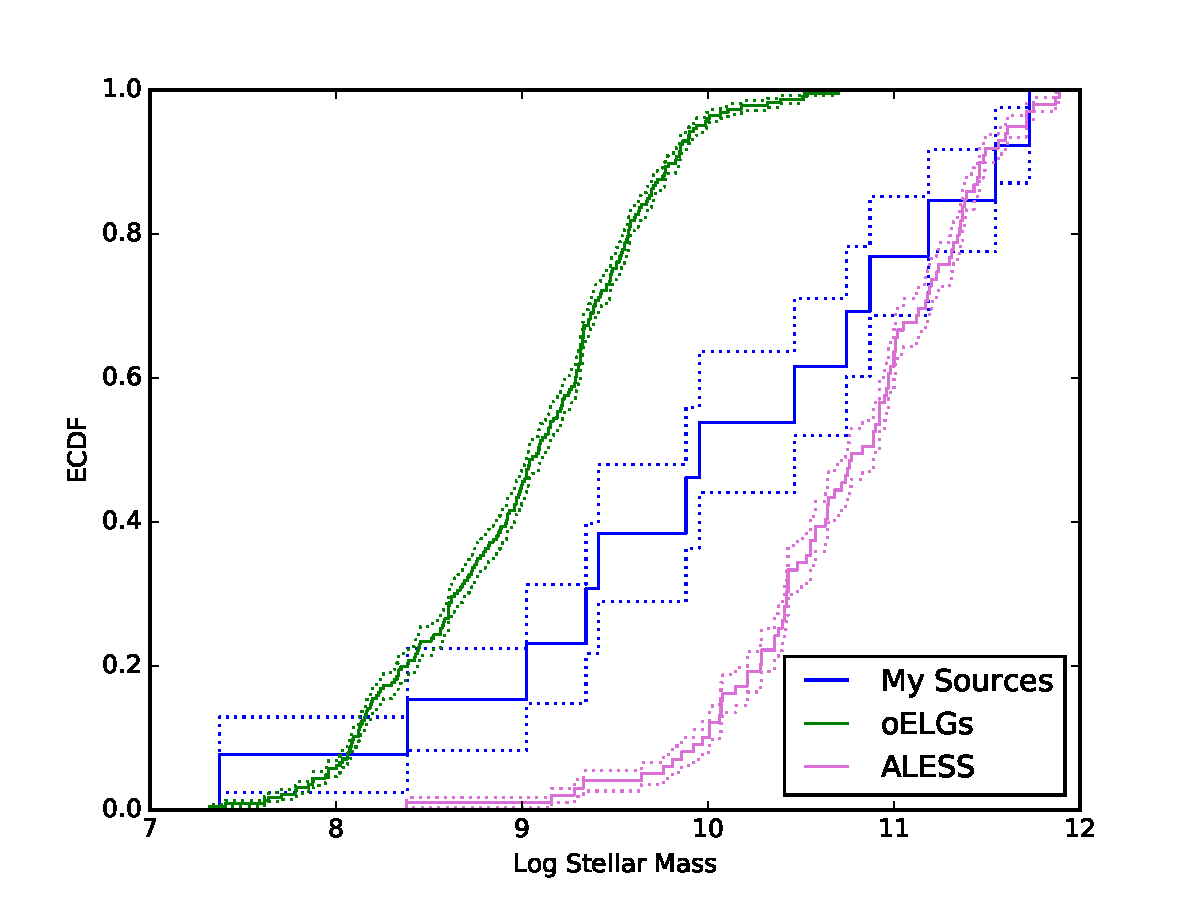
\includegraphics[scale=0.8]{ecdf_mass.pdf}
\caption{Stellar mass comparison between our serendipitously selected sub-mm galaxies and our four comparison samples. We see that our sample is bracketed by the comparison samples. Our galaxies cover a very wide range of $4+$ dex in stellar mass. Our galaxies match best with the sample from \cite{dunlop16}. Some are very massive in line with the ALESS sample, while others more than one dex less massive than any ALESS galaxy are far more similar to the low mass oELG sample.}
\label{fig:mass_comp}
\end{figure}

Figure \ref{fig:sfr_comp} shows star formation rate comparison between our galaxy sample and the comparison samples. We again note the similarities between our sample and the \cite{dunlop16} sample. This is reasonable considering the detection technique, serendipitous ALMA detections, are very similar. Also note that our sample is bracketed by the more traditional starbursting SMGs of the ALESS sample, and the lower star formation rates (from less massive galaxies) in the oELG and K16 samples.

\begin{figure}[t]
\centering
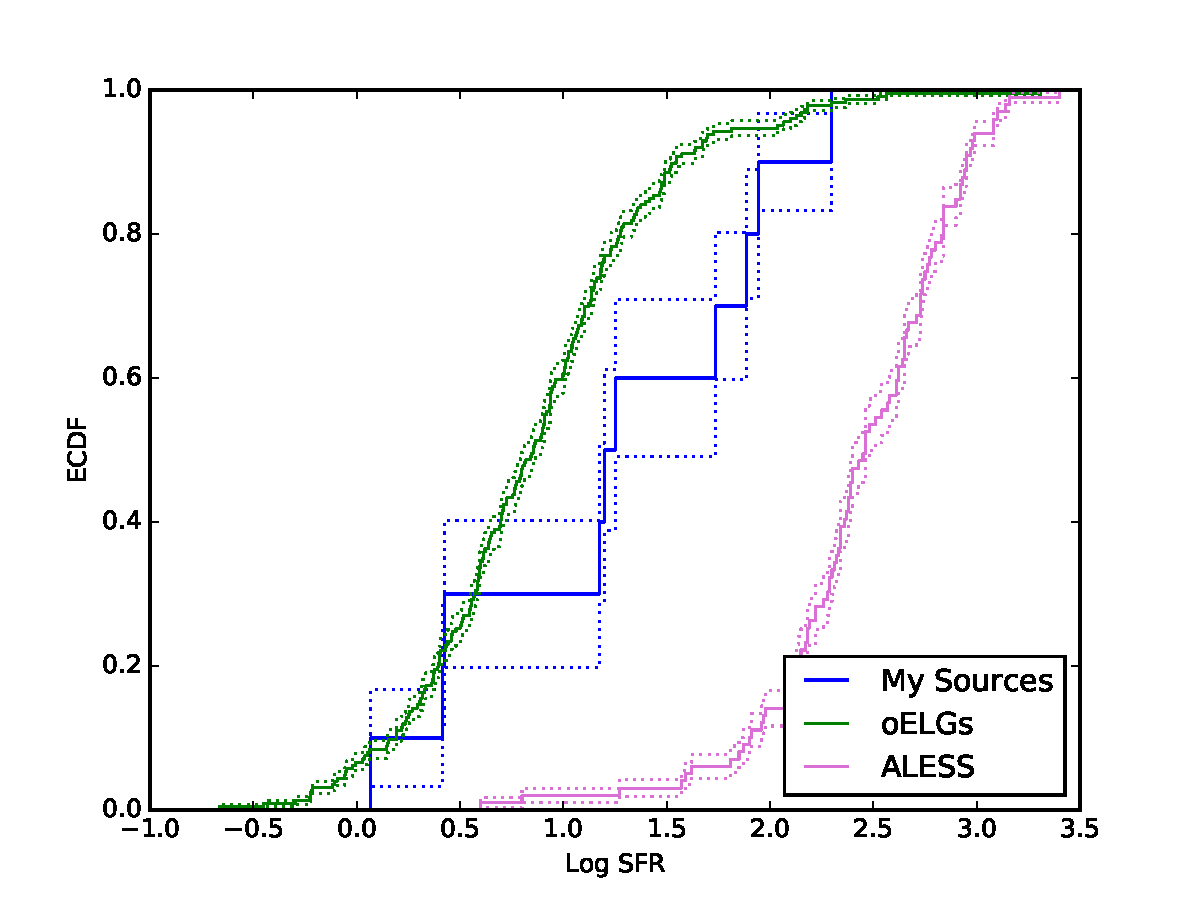
\includegraphics[scale=0.8]{ecdf_sfr.pdf}
\caption{Star formation rate comparison between our sample and the four comparison samples. We match very well with the D16 sample. The ALESS sample is made up of more massive, higher SFR galaxies, while the oELG and K16 samples are lower SFR due to their lower masses.}
\label{fig:sfr_comp}
\end{figure}

Comparison of the dust attenuation, dust to stellar mass ratio, and the dust temperature are found in Figures \ref{fig:av_comp}, \ref{fig:mstar_mdust}, \& \ref{fig:tdust}, respectively. The attenuation comparison again demonstrates how some physical properties of our sample match well with the D16 sample, and are bracketed between the oELG and ALESS samples. Our galaxies have slightly more dust than the oELGs, with a median $A_V = 1$, but they don't go to the very high $A_V$ of 5 or more as seen in the tail of the ALESS sample. In the comparison of the dust mass to stellar mass ratio in Figure \ref{fig:mstar_mdust}, we see that our serendipitously selected galaxies extend to one dex lower dust to stellar mass ratios than the ALESS sample. Others in our sample match the ALESS sample quite well in this respect, though, again showing the diversity and range of physical properties of this sample. The dust temperature comparison in Figure \ref{fig:tdust} shows that the luminosity weighted dust temperature of both our sample and the ALESS samples have approximately the same range. However, our sample has a much different distribution, although this could easily be due to small number statistics. The best fit cold dust temperature for all our galaxies is $\sim 25$K. The fraction of higher $T_{Dust}$ temperatures compared to ALESS is most likely due to a large fraction of the dust luminosity coming from the warm dust in star forming regions.

\begin{figure}[t]
\centering
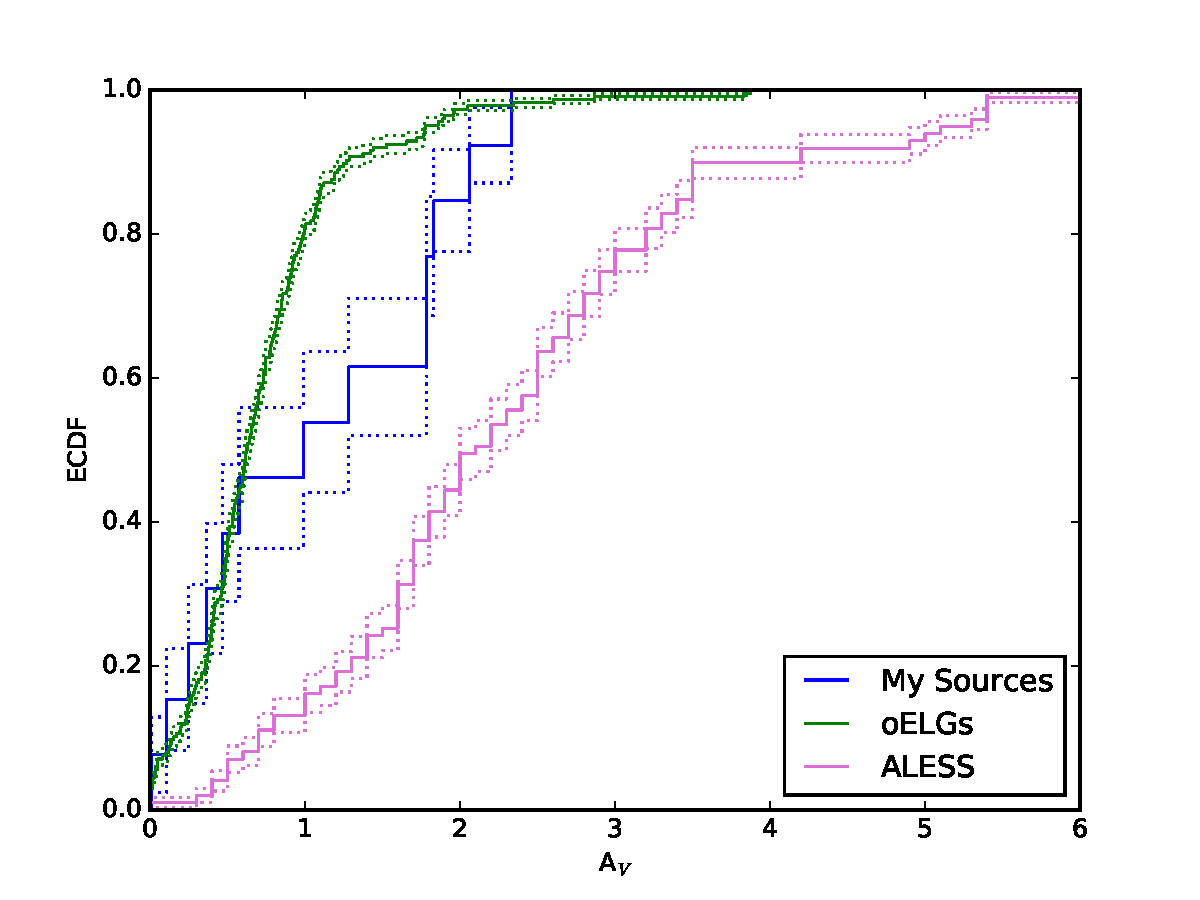
\includegraphics[scale=0.8]{ecdf_av.pdf}
\caption{$A_V$ comparison between our sample and  comparison samples. We again match the D16 sample very well. As with Figure \ref{fig:mass_comp}, our sample is bracketed between the ALESS and oELG samples. The dust attenuation properties of our sample range from high $A_V$ to very low $A_V$, again demonstrating the large variety of physical properties found in our galaxy sample.}
\label{fig:av_comp}
\end{figure}

\begin{figure}[t]
\centering
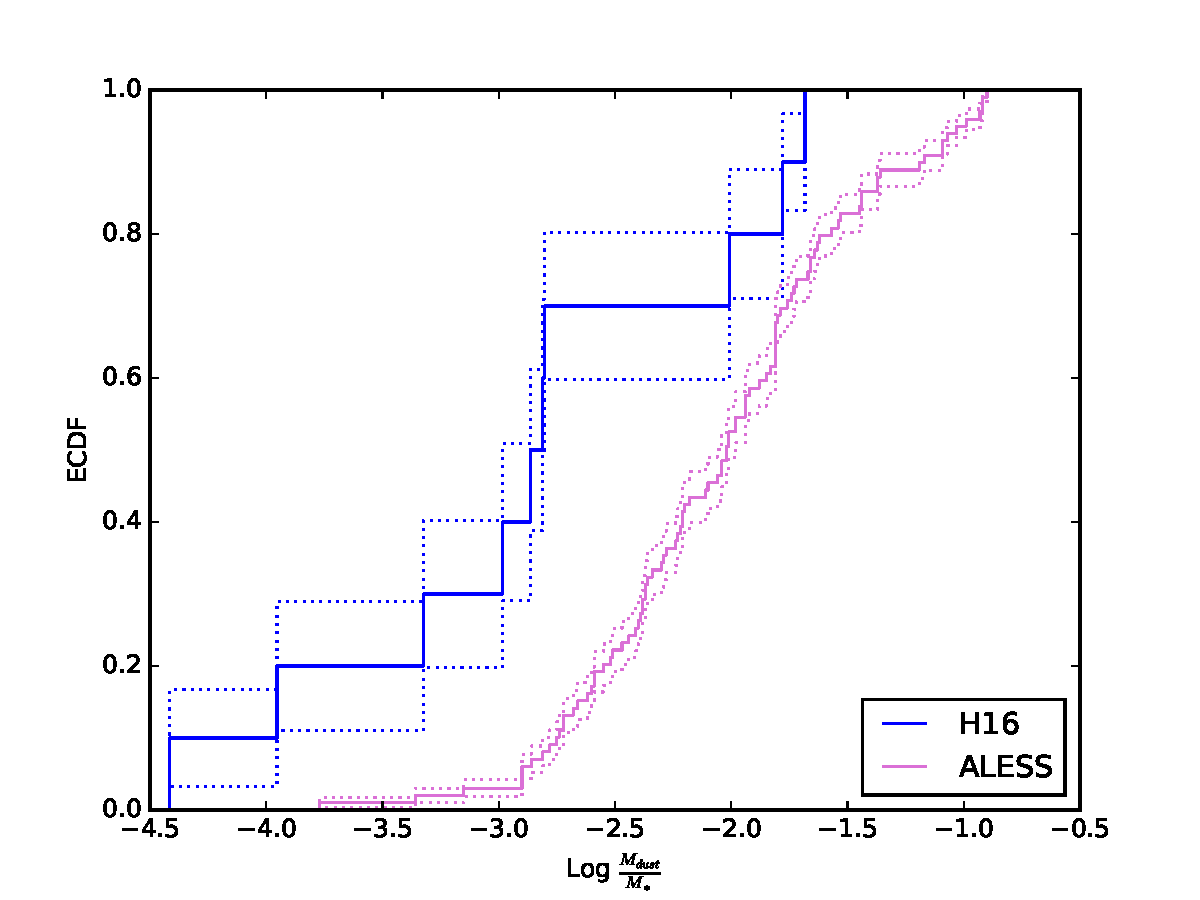
\includegraphics[scale=0.8]{ecdf_mdust_mstar.pdf}
\caption{Dust to stellar mass comparison between our sample and the ALESS sample. As in the comparison of $A_V$, Figure \ref{fig:av_comp}, our galaxies can be significantly more dust poor than ALESS galaxies.}
\label{fig:mstar_mdust}
\end{figure}

\begin{figure}[t]
\centering
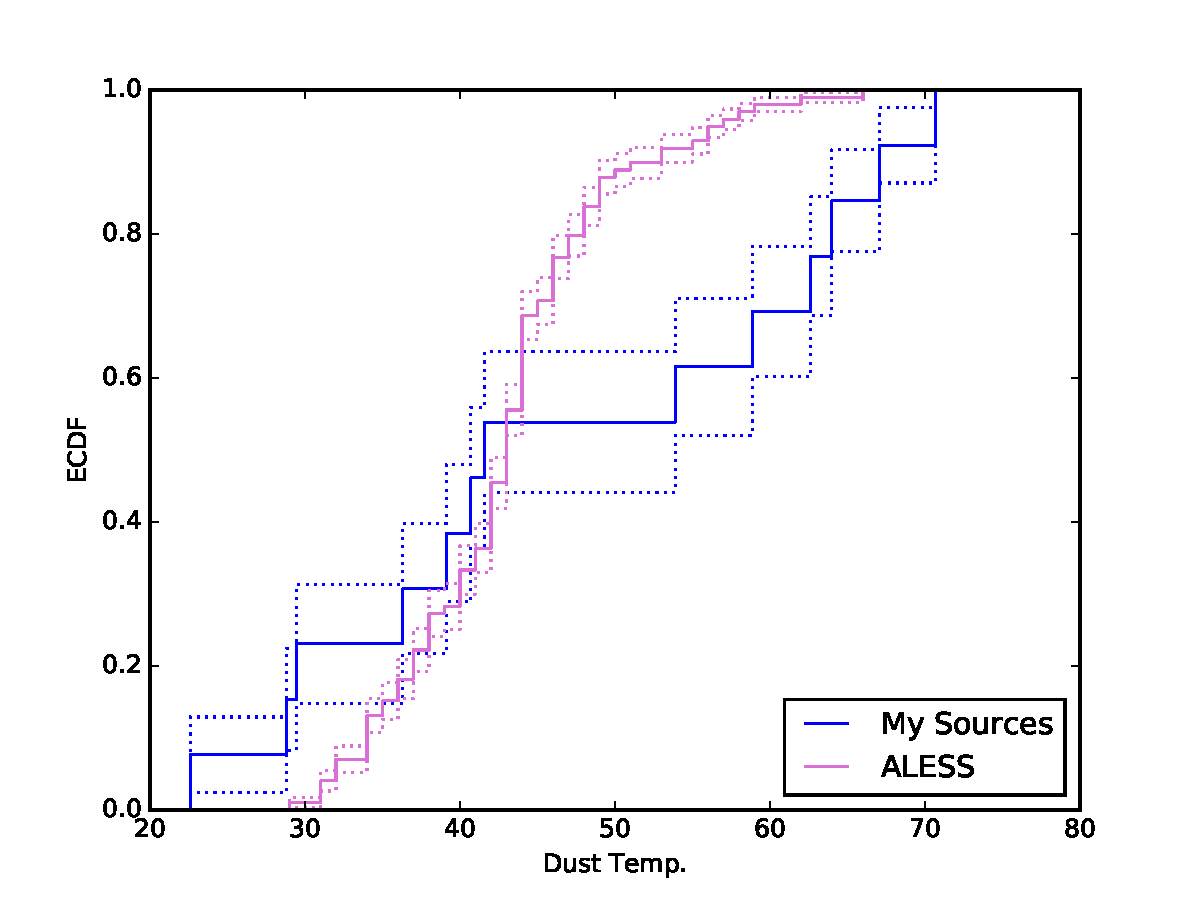
\includegraphics[scale=0.8]{ecdf_tdust.pdf}
\caption{Dust temperature comparison between our sample and the ALESS sample. Note that $T_{Dust}$ is the luminosity weighted dust temperature (see equation 8 of \cite{dacunha15}), and not the cold dust temperature. The ranges of both galaxy samples are approximately the same, though there is a possible multimodality of our serendipitous sample; a larger sample would be needed to explore this more concretely.}
\label{fig:tdust}
\end{figure}

\subsection{Stellar Mass--Star Formation Rate Relation}

Figure \ref{fig:mainseq} shows our sample and the comparison samples on the stellar mass --- star formation rate relation. We also add in 4 additional SMGs from \cite{yamaguchi16} as well as best fit stellar mass -- SFR relations from \cite{speagle14} at $z = 2.5, 2.0, and 1.5$. Additionally, we split our sample into different redshift bins to best interpret this figure.  We note that our galaxies, as well as those from D16, lie on the SM -- SFR relation as defined by continuum and emission line sources. Our lower redshift sources are below this relation as would be expected.

\begin{figure}[t]
\centering
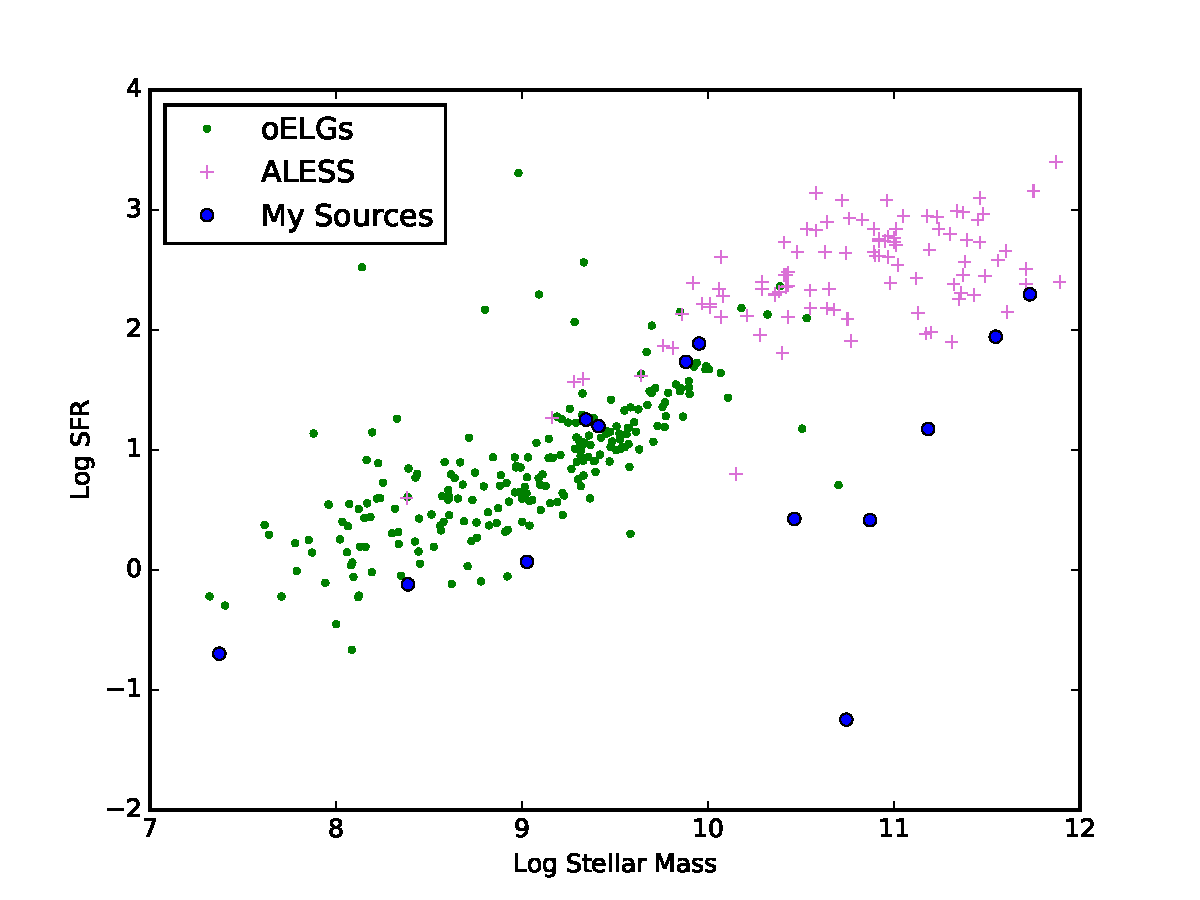
\includegraphics[scale=0.8]{main_seq.pdf}
\caption{Stellar mass -- star formation rate relation. The lines are from \cite{speagle14} at $z = 2.5, 2.0, and 1.5$. Our seredipitously selected ALMA sources lie on the main sequence as defined by continuum and emission line selected sources.}
\label{fig:mainseq}
\end{figure}

%\subsection{Object of Particular Interest: A1}


\section{Conclusion}
\label{sec:conclusion}

This work demonstrates that selecting serendipitous sub-mm sources results in galaxies with a wide range of physical properties. They are not simple scaled versions of SMGs, and instead have a large range of attenuations and dust properties. As ALMA continues to provide new deep imaging in fields covered with \textit{HST} and other telescopes, studying the serendipitously discovered ALMA source provides for a way to probe across a wide range of physical properties. While this sample is limited in its size, future ALMA observations should provide hundreds of these galaxies in fields with ancillary photometry.

\acknowledgments
\section*{Acknowledgments}
Based in part on observations made with the NASA/ESA Hubble Space Telescope, 
and obtained from the Hubble Legacy Archive, which is a collaboration between
the Space Telescope Science Institute (STScI/NASA), the Space Telescope 
European Coordinating Facility (ST-ECF/ESAC/ESA) and the 
Canadian Astronomy Data Centre (CADC/NRC/CSA). 
This work is based in part on observations made with the Spitzer Space Telescope, 
which is operated by the Jet Propulsion Laboratory, California Institute of Technology under a contract with NASA.
This research has made use of data from HerMES project (\url{http://hermes.sussex.ac.uk/}). 
HerMES is a Herschel Key Program utilizing Guaranteed Time from the SPIRE instrument team,
ESAC scientists and a mission scientist.
The HerMES data was accessed through the Herschel Database in 
Marseille (HeDaM - \url{http://hedam.lam.fr}) operated by CeSAM and
hosted by the Laboratoire d'Astrophysique de Marseille.

Funding for the SDSS and SDSS-II has been provided by the Alfred P. Sloan Foundation, 
the Participating Institutions, the National Science Foundation, the U.S. Department of Energy, 
the National Aeronautics and Space Administration, the Japanese Monbukagakusho, 
the Max Planck Society, and the Higher Education Funding Council for England. 
The SDSS Web Site is \url{http://www.sdss.org/.}
Funding for SDSS-III has been provided by the Alfred P. Sloan Foundation, the Participating Institutions, 
the National Science Foundation, and the U.S. Department of Energy Office of Science. 
The SDSS-III web site is \url{http://www.sdss3.org/}.

This research has made use of NASA's Astrophysics Data System.
This research has made use of the NASA/ IPAC Infrared Science Archive, 
which is operated by the Jet Propulsion Laboratory, California Institute of Technology, 
under contract with the National Aeronautics and Space Administration.
%This research has made use of the NASA/IPAC Extragalactic Database (NED), 
%which is operated by the Jet Propulsion Laboratory, California Institute of Technology, 
%under contract with the National Aeronautics and Space Administration.
%This research has made use of the VizieR catalogue access tool, CDS,
%Strasbourg, France. The original description of the VizieR service was
%published in \cite{vizier}.

The Institute for Gravitation and the Cosmos is 
supported by the Eberly College of Science and the Office of the Senior Vice
President for Research at the Pennsylvania 
State University. This research has made use of NASA's Astrophysics Data System 
and the python packages \texttt{IPython}, \texttt{AstroPy}, 
\texttt{NumPy}, \texttt{SciPy}, \texttt{scikit-learn}, and \texttt{matplotlib}
 \citep{ipython, astropy, numpy, scipy, scikit-learn, matplotlib}.

I am very grateful to my spouse, friend, and future parenting partner, Lea M.Z. Hagen.

\bibliographystyle{apj}                       %% AASTeX
\bibliography{mybib}

\end{document}
